%!TEX root = ../dissertation.tex

\section*{Общая характеристика работы} %\addcontentsline{toc}{section}{Общая характеристика работы}

%!TEX root = ../dissertation.tex

\nociteallauthorpublicationsmaindocument

\textbf{Актуальность темы исследования.}  
В задачах прикладной математики и информатики часто требуется формальное описание и количественная оценка различий между сложными дискретными структурами --- перестановками, графами и деревьями, а также анализ процесса эволюции во времени этих структур~\cite{Penny2004,Bunke1997}.  
Подобные задачи возникают в разных областях: от изучения аудиовизуальной и текстовой информации до моделирования социальных сетей и сопоставления топологий~\cite{baret2004phylogenetic,McCollum2023,Piar2020,Newman2003}.  
Классическим примером является вычисление ``расстояния'' между двумя перестановками (минимального числа операций, переводящих одну конфигурацию в другую), что лежит в основе алгоритмов сортировки перестановок, анализа редактирования графов (англ. \textit{graph edit distance}), а также ряда других задач структурного сравнения~\cite{Pevzner03}.  

Однако, когда речь заходит о процессе изменений, ситуацию усложняет тот факт, что операции над структурой (добавление рёбер в графы, перестановки элементов, модификации вершин дерева) могут происходить случайным образом с неоднородными вероятностями.  
В одних случаях вероятность операции считается одинаковой для всех элементов, как в классической модели \mbox{Эрдёша--Реньи} (равновероятное появление рёбер)~\cite{Erdos1959}, в других же требуется учесть разные ``аффинности'' отдельных элементов.  
Такое неравномерное распределение вероятностей оказывается востребованным при моделировании социальных сетей, процессов обработки и передачи информации, соавторства текстов, взаимодействия порядка генов и т.~п.  

Кроме того, ещё одной важной проблемой является обнаружение параллельных (независимых) изменений в процессах на древовидном пространстве состояний.  
Если в вершинах дерева находятся разные версии исходного объекта (программного кода, текстовой традиции, биологической структуры и т.~д.), то нередко интересуют изменения, которые возникли неоднократно и независимо друг от друга на разных ветвях дерева.  
Подобные конвергентные события важно выявлять в лингвистике (одинаковые языковые новации в независимых группах), в программной инженерии (одинаковые ``патчи'', реализованные параллельно), а также в биологии (повторные мутации в разных популяциях)~\cite{Rokas2008}.  
Ранняя (парсимонийная) техника анализа обычно фиксирует минимальное число изменений, не давая количественной меры, отражающей степень параллельности.  
Проблема усложняется, если число различных ветвей велико, и требуется формализованная методика с ранжированием по ``важности''. 

Биологические приложения занимают особое место в перечисленных задачах.  
Эволюционные изменения геномов можно рассматривать как особый вид информационных процессов, в ходе которых происходят сложные преобразования структурной организации генетической информации. 
Количество таких операций изменения между двумя видами часто служит мерой эволюционной дистанции между ними. 
При сравнении и эволюции геномов блоки (гены) можно рассматривать как перестановки, и расстояние между ними (количество инверсий или транспозиций) даёт оценку эволюционной близости~\cite{yancopoulos2005,braga2010}.  
При описании взаимодействий генов или клеточных состояний удобно использовать случайные графы, причём требуются модели, учитывающие различную ``интенсивность'' связей~\cite{Barabsi2004}. 
Такие обобщённые модели (с аффинностями) могут предсказывать появление ``гигантской компоненты'' при иных порогах, чем классическая модель Эрдёша--Реньи. 
Это существенно влияет на интерпретацию биологических данных, когда слишком упрощённая модель недооценивает или переоценивает вероятность ``слияния'' крупных фрагментов в эволюционном процессе~\cite{tannier2016}.  

Таким образом, актуальными и востребованными \textbf{задачами} являются:  
\begin{enumerate}
    \item разработка и анализ процессов случайных операций над дискретными структурами с неоднородными вероятностями;  
    \item оценка расстояния между конфигурациями с возможностью достоверно учитывать крупные масштабы изменений;  
    \item автоматизации анализа параллельных изменений на деревьях и введении количественных метрик степени их независимого возникновения. 
\end{enumerate}

\textbf{Степень разработки проблемы.}  
Разнообразные аспекты сравнения и эволюции дискретных структур были изучены в ряде фундаментальных и прикладных исследований.  

Случайные графы и их обобщения. 
Классическая модель Эрдёша--Реньи, в процессе измениния которой каждое ребро добаляется с одинаковой вероятностью, нашла широкое применение, описаное, в частности, в работах А.М.~Райгородского~\cite{райгородский2010модели,райгородский2022модели}.  
Позднее было показано, что во многих реальных сетях (социальных, биологических) важно учитывать неоднородность ``аффинностей'' вершин~\cite{tannier2016}.
Данные обобщения позволяют точнее описывать системы с дифференцированным вкладом узлов.
Однако итоговые формулы (например, для порога появления гигантской компоненты) сложны в вычеслении и применении и требуют новых комбинаторных и аналитических результатов~\cite{tannier2016}.  

Сравнение перестановок и вычисление расстояний.
Для описания процесса изменения последовательностей (в том числе геномных) широко применяются метрики на перестановках.
Уже в 1990-х были сформулированы методы вычисления расстояния перестановок (например, через минимальное число операций инверсии/транспозиции)~\cite{yancopoulos2005,braga2010}, а также предложены статистические модели случайных перестроек (DCJ-модель, модель ``хрупких'' регионов)~\cite{Pevzner03,tannier2016}.
Тем не менее, существующие подходы нередко опираются на бесконечные рядовые разложения и трудоёмкие итерационные алгоритмы, которые становятся неустойчивыми при большом количестве изменений~\cite{tannier2016}.
Это затрудняет оценку истинной дистанции и требует поиска новых аналитических решений.  

Обнаружение параллельных изменений на деревьях.
В филогенетическом анализе, а также при изучении версий ПО, культурных традиций и других ``древовидных'' процессах, давно известно, что один и тот же признак (исправление фрагмента кода, мутация, вставка текста и т.~п.) может возникать неоднократно и независимо.  
Методы парсимонии (например, алгоритм Фитча) выявляют минимальное число таких изменений, но не дают количественной меры параллельности~\cite{Avdeyev2016}.
Ранние решения были фрагментарными и использовались, в основном, вручную, когда исследователь сам отмечает ``зоны повторного возникновения''. 
Строгое формальное описание и автоматизация подобного анализа остаются открытой проблемой, особенно при больших масштабах данных.  

Таким образом, к настоящему моменту накоплен значимый теоретический и прикладной инструментарий для исследования случайных дискретных структур, оценки расстояний и анализа эволюционных деревьев.  
Однако существенные ограничения всё ещё сохраняются:

\begin{itemize}
    \item Неоднородность вероятностей далеко не всегда учитывается в традиционных моделях (например, классической модели Эрдёша--Реньи). При этом реальные системы (биологические, социальные) часто требуют более гибких параметров;  
    \item Вычислительная сложность и расходимость рядов в существующих вероятностных моделях для перестановок и графов затрудняют получение точных оценок расстояния при больших масштабах изменений;  
    \item Отсутствие формализованных алгоритмов выявления и количественной оценки параллельных изменений на деревьях: минимальное объяснение парсимонии не отражает ``степень'' и распределённость независимых появлений признака.  
\end{itemize}

Всё это указывает на необходимость разработки новых алгоритмов обработки данных, позволяющих (1) строить обобщённые случайные модели с учётом неоднородных вероятностей, (2) выводить аналитические формулы для расчёта расстояний, преодолевающие проблемы бесконечных рядов, и (3) автоматизировать обнаружение параллельных изменений с количественной оценкой их ``независимости''.  
Результаты таких исследований востребованы как в теоретической математике (расширение классических моделей и методов комбинаторного анализа), так и в прикладных исследованиях, особенно в задачах эволюционной биологии, но и за её пределами --- в лингвистике, анализе версий ПО, культурно-исторических исследованиях и других сферах.  

\textbf{Научная новизна} состоит в том, что: 
(1) впервые получены аналитические выражения для оценки числа компонент в рамках случайных графов с индивидуальными вероятностями (обобщение модели Эрдёша--Реньи), устраняющие необходимость численного суммирования расходящихся рядов.
(2) найден порог появления гигантской компоненты в модели случайных графов с неравномерными аффинностями, что вдвое меньше порога в классической модели Эрдёша–Реньи.
(3) разработан метод оценки истинного расстояния между двумя конфигурациями с учётом неоднородностей, позволяющий устойчиво вычислять метрику при высоком уровне перестроек. 
(4) предложен алгоритм автоматического выявления параллельных изменений на деревьях. 
Введена новая комбинаторная метрика параллельности, позволяющая ранжировать независимые события по степени их распределённости на разных ветвях.


\textbf{Теоретическая значимость} определяется расширением классических вероятностных постановок путём введения неоднородных вероятностей, а также количественной формализацией параллельных изменений на деревьях.  
В частности: (1) получены новые комбинаторные и асимптотические результаты, описывающие ожидаемое количество компонент заданного размера и появление гигантской компоненты для графов с индивидуальными аффинностями вершин; 
(2) предложены метод оценки расстояний между перестановками при больших масштабах изменений;
(3) систематизирован подход к ранжированию случаев независимых изменений в древовидной топологии.

\textbf{Практическая значимость работы} определяется:

\begin{enumerate}
    \item Повышение точности оценки расстояний при больших больших масштабах изменений, что важно для сравнительного анализа геномов, крупных текстовых данных.
    \item Автоматизированная идентификация и ранжирование параллельных (независимых) изменений, востребованная в биоинформатике (выявление конвергентных мутаций), лингвистике (одинаковые инновации в родственных языках) и др.
    \item Программная реализация (пакет \emph{TruEst} для вычисления расстояний и \emph{PaReBrick} для обнаружения параллельных событий), открытая для интеграции в другие исследовательские инструменты.
\end{enumerate}

\textbf{На защиту выносятся положения, обладающие научной новизной:}
\begin{enumerate}[label={\arabic*.}]
    \item Комбинаторный метод описания процесса изменения случайных графов с неравномерными аффинностями (обобщающий классическую модель Эрдеша-Реньи), отличающийся тем, что, с целью корректного учёта неоднородных вероятностей рёбер, предложены аналитические формулы для оценки числа компонент связности заданного размера и доказан новый порог появления гигантской компоненты, что расширяет применимость модели.
    \item Алгоритм оценки расстояния между объектами, представленными перестановками на основе случайных графов с неоднородными вероятностями состояний, отличающийся тем, что, с целью повышения точности вычислений на больших расстояниях, вместо численного суммирования потенциально расходящихся рядов используются аналитические выражения для ключевых характеристик циклограммы перестановки, что позволило реализовать устойчивое вычисление расстояния даже при высоком уровне эволюционных изменений.
    \item Алгоритм выявления и ранжирования независимых изменений в процессах эволюции наборов перестановок на древовидных информационных структурах, отличающийся тем, что, с целью автоматического и объективного обнаружения повторяющихся (конвергентных) событий в информационных процессах, вводится новая комбинаторная метрика — «показатель параллельности», количественно отражающая как частоту и количество независимых изменений, так и их распределённость по вершинам дерева, что повышает достоверность и наглядность анализа параллельных эволюционных изменений.
\end{enumerate}

\textbf{Методы исследования.} 
В работе использованы методы теории вероятностей и математической статистики, комбинаторные методы и алгоритмы на деревьях, методы численной оптимизации и анализа сходимости, экспериментальные тесты на синтетических и реальных данных (в первую очередь, геномных), оценивающие точность и скорость разработанных алгоритмов.

\textbf{Достоверность} научных результатов обеспечена: строгими математическими доказательствами корректности полученных формул, валидацией на симулированных данных, где истинные параметры известны заранее, сравнением с опубликованными результатами и моделями (включая классические алгоритмы оценки расстояния по перестановкам), открытым доступом к программному коду (\texttt{GitHub}-репозитории \emph{TruEst} и \emph{PaReBrick}), позволяющим независимо воспроизвести эксперименты.

\textbf{Соответствие паспорту специальности.}
Полученные научные результаты соответствуют следующим пунктам паспорта специальности 2.3.8~--- ``Информатика и информационные процессы (технические науки)'':

\textbf{Пункт 1}~--— ``Разработка компьютерных методов и моделей описания, оценки и оптимизации информационных процессов и ресурсов, а также средств анализа и выявления закономерностей на основе обмена информациейпользователями и возможностей используемого программно-аппаратного обеспечения''.
Разработаны компьютерные методы описания и оптимизации информационных процессов изменения дискретных структур (перестановок и графов) с учётом неоднородных вероятностей.;

\textbf{Пункт 4}~--— ``Разработка методов и технологий цифровой обработки аудиовизуальной информации с целью обнаружения закономерностей в данных, включая обработку текстовых и иных изображений, видео контента. Разработка методов и моделей распознавания, понимания и синтеза речи, принципов и методов извлечения требуемой информации из текстов.''.
Разработаны методы и алгоритмы обработки и анализа информации, включая автоматизированный анализ параллельных изменений.

% \textbf{Пункт 7}~--— ``Разработка методов обработки, группировки и аннотирования информации, в том числе, извлеченной из сети интернет, для систем поддержки принятия решений, интеллектуального поиска, анализа''.
% Предложены алгоритмы автоматизированной обработки и группировки информации, полученной из различных источников.

\textbf{Апробация результатов работы}

Основные результаты работы были представлены на следующих  конференциях:

\begin{itemize}
    \item RECOMB Comparative Genomics, 2022, онлайн;
    \item XI Конгресс молодых ученых, 2022, Университет ИТМО, Санкт-Петербург, Россия;
    \item Moscow Conference on Computational Molecular Biology, 2021, Москва, Россия;
    \item Пятидесятая научная и учебно-методическая конференция, 2021, Университет ИТМО, Санкт-Петербург, Россия;
    \item BiATA 2020 (Bioinformatics: From Algorithms to Applications), 2020, онлайн;
    \item RECOMB Comparative Genomics (постерный доклад), 2019, Монтпелье, Франция;
    \item Вероятностные методы в дискретной математике, 2019, Петрозаводск, Россия;
    \item Moscow Conference on Computational Molecular Biology, 2019, Москва, Россия;
    \item RECOMB Comparative Genomics, 2018, Шербрук, Канада;
\end{itemize}

\newpage

\section*{СОДЕРЖАНИЕ РАБОТЫ}

Во \textbf{введении} обоснована актуальность научных исследований, проводимых в рамках данной диссертационной работы, описана степень разработки проблемы вывода демографической истории популяций по генетическим данным, обзор методов моделирования демографических историй, сформулированы цели и задачи, описаны научная новизна, теоретическая и практическая значимости работы, а также перечислены положения, выносимые на защиту.

В \underline{\textbf{первой главе}} приводится обзор предметной области, который включает определение демографической истории популяций, описание существующих методов вывода демографических историй популяций по генетическим данным.

В \textbf{разделе~1.1} описаны основные определения популяционной генетики, используемые в данной работе.
Она включает формальное определение демографической истории популяций.
Популяционная генетика является важной областью генетики, изучающей изменение генетического состава популяций и их эволюцию.
Она решает такие задачи, как определение структуры популяций, построение филогенетических деревьев и поиск демографической истории популяций.

%\emph{Популяция} --- это группа организмов одного вида, находящихся в определенной географической области и взаимодействующих друг с другом
%\emph{Эффективный размер популяции} $N_e$ --- это концепт, используемый для описания того, какой размер имела бы идеальная популяция с таким же уровнем генетического разнообразия, как и реальная популяция.
%Эффективный размер популяции $N_e$ обычно меньше, чем фактический размер популяции, однако, все же является более важной характеристикой популяции.
%\emph{Инбридинг} --- это образование потомства в результате размножения близкородственных особей.
%Он измеряется коэффициентом инбридинга, который отражает  степень близкородственных связей.

\emph{Демографическая история популяций} --- история эволюции и развития популяций, которая включает в себя информацию о том, как популяции делились и образовывались, какова была численность популяций, интенсивность миграции, \textit{коэффициенты инбридинга} --- степень близкородственных связей, и много другого.
Примеры визуального представления демографических историй представлены на рисунке~\ref{fig:syn_rus:dem_inf:dem_his_examples}.
Информация о численности популяций и миграциях отображена шириной закрашенных областей и стрелками между ними.
Время в демографических историях зачастую измеряется в поколениях или годах и отображено по оси ординат.
%Под \textit{численностью или размером популяции} в демографической истории понимается эффективный размер популяции --- концепт популяционной генетики, используемый для описания того, какой размер имела бы идеальная популяция с таким же уровнем генетического разнообразия, как и реальная популяция.
 
\begin{figure}[b]
    \centering
    \begin{subfigure}[b]{.33\textwidth}
    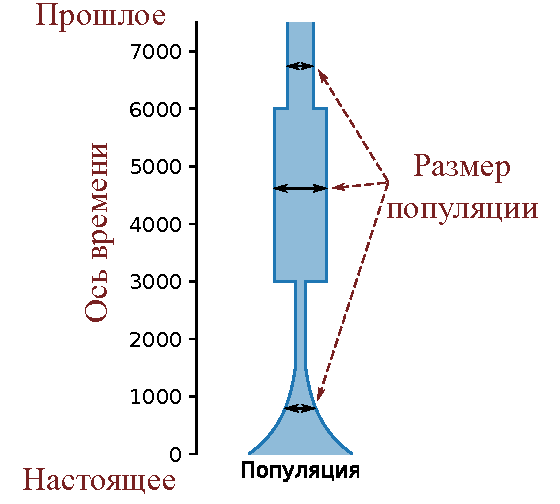
\includegraphics[width=\textwidth]{images/part1/dem_history/1d_model_fixed.pdf}
    \caption{}
    \labelsyn{fig:syn_rus:dem_inf:dem_his_examples_1}
    \end{subfigure}%
    \begin{subfigure}[b]{.33\textwidth}
    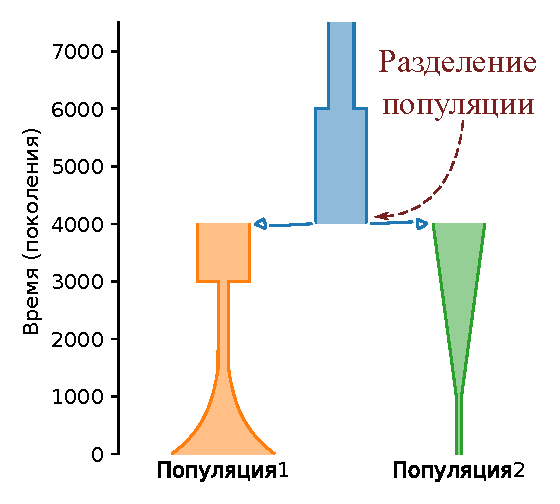
\includegraphics[width=\textwidth]{images/part1/dem_history/2d_model_isolation_fixed.pdf}
    \caption{}
    \labelsyn{fig:syn_rus:dem_inf:dem_his_examples_2}
    \end{subfigure}%
    \begin{subfigure}[b]{.33\textwidth}
    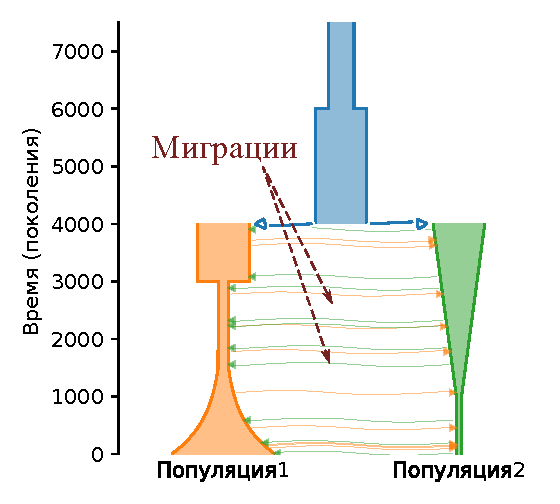
\includegraphics[width=\textwidth]{images/part1/dem_history/2d_model_migration_fixed.pdf}
    \caption{}
    \labelsyn{fig:syn_rus:dem_inf:dem_his_examples_3}
    \end{subfigure}
    \caption{Примеры визуального представления демографических историй одной и двух популяций}
    \labelsyn{fig:syn_rus:dem_inf:dem_his_examples}
\end{figure}

% В современной литературе нет определенности со строгим определением демографической истории.
% Приведем формальное определение демографической истории популяций, которое будет использовано в данной работе.

% \definition Демографическая история $\mathcal{D}$ для $P$ популяций --- это четверка ${\langle T, \mathfrak{G}, \mathfrak{M}, \mathcal{C} \rangle}$, где ${T = \langle V, E \rangle}$ --- полное бинарное дерево, в котором вершины ассоциированы с популяциями и которое определяет структуру разделения популяций, ${\mathfrak{G}: V \to \mathbb{R}_+ \times \mathbb{R}_+ \times \mathcal{F}_{\mathbb{R}_+ \to \mathbb{R}_+}}$ --- отображение, которое для каждой вершины~$v$ ставит в соответствие множество ${\langle t_v, t^d_v, g(t) \rangle}$, где $t_v$ и $t^d_v$ --- время образования и разделения популяции~$v$ соответственно, а функция ${g(t): [t_v, t^d_v] \to \mathbb{R}_+}$ определяет численность популяции в каждый момент ее существования, а ${\mathfrak{M} = \{\mathfrak{M}_q\},\ \mathfrak{M}_q \in \widetilde{\mathscr{M}} \cup \mathscr{M}}$ --- набор единичных и непрерывных миграций, $\mathcal{C}: V \to \mathbb{R}^C$ --- набор дополнительных констант для популяций.

% На отображение $\mathfrak{G}$ накладывается следующее ограничение: для любой вершины $v$ время ее образования $t_v$ равно времени разделения $t^d_{parent(v)}$ ее вершины-родителя.
% Для любой единичной миграции ${\mathfrak{M}_q = \langle v_1, v_2, t, m \rangle}$ выполняется: ${v_1, v_2 \in V}$ и $t \in [t_{v_1}, t^d_{v_1}] \cap [t_{v_2}, t^d_{v_2}]$.
% Для любой непрерывной миграции ${\mathfrak{M}_q = \langle v_1, v_2, t^s, t^e, m \rangle}$ выполняется: ${v_1, v_2 \in V}$ и ${t^s, t^e \in [t_{v_1}, t^d_{v_1}] \cap [t_{v_2}, t^d_{v_2}]}$.
% В качестве дополнительных констант для популяций в данной работе будут рассмотрены коэффициенты инбридинга $\mathcal{C}(v_i) = F_i,\ i=1,\ldots,P$, заданные для листьев $\{v_i\}_{i=1}^P$ дерева $T$.

% Рисунок~\ref{fig:syn:dem_def} демонстрирует пример демографической истории популяций как набора из дерева разделений, отображения на его вершинах, множества миграций и констант.

% \begin{figure}[ht]
%     \centering
%     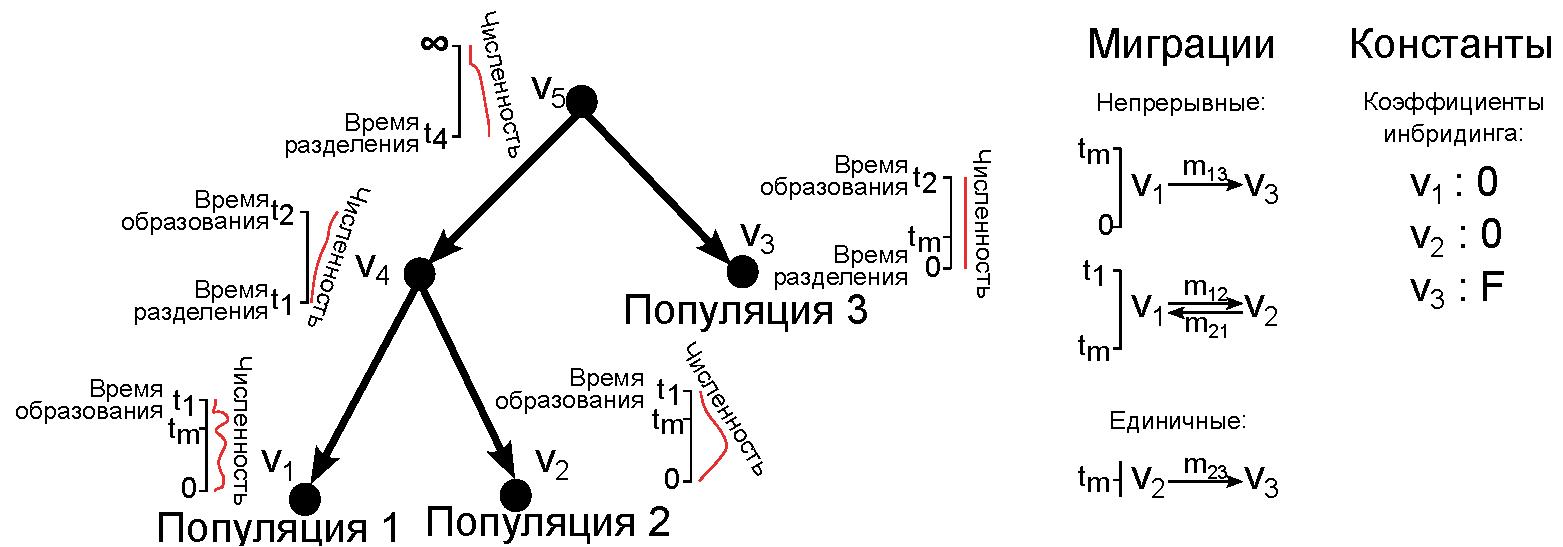
\includegraphics[width=0.9\textwidth]{images_2/dem_hist_def.pdf}
%     \caption{Пример демографической истории популяций как множества из дерева разделений с заданными временами и функциями численности, набора миграций и дополнительных констант}
%     \labelsyn{fig:syn:dem_def}
% \end{figure}



\newpage
В \textbf{разделе 1.2} описана постановка задачи вывода демографической истории популяций по генетическим данным с использованием параметрических моделей, а также описаны основные компоненты существующих методов решения этой задачи.
В разделе приведено краткое описание известных программных средств, реализующих эти методы, а именно \dadi, \moments, \momi и \momentsLD.

Для вывода демографической истории популяций используются параметрические модели, которые представляют собой \textit{метрические деревья с функциями на ребрах}.
Использование моделей позволяет, во-первых, ограничить пространство поиска, а, во-вторых, использовать методы оптимизации для настройки значений их параметров по генетическим данным.
На рисунке~\ref{fig:model_def2} изображен пример модели в виде метрического дерева с функциями на ребрах, которое описывает демографическую историю двух популяций.

\begin{figure}[ht]
    \centering
    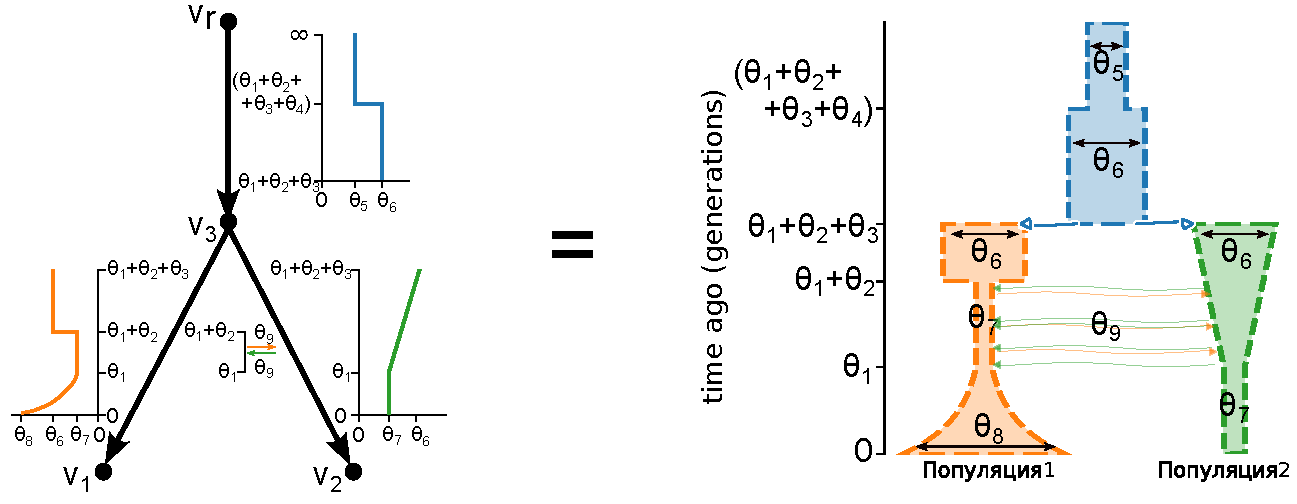
\includegraphics[width=0.7\textwidth]{images/part1/2d_model_metric_tree_2.pdf}
    \caption{Пример модели демографической истории двух популяции в виде метрического дерева с функциями на ребрах}
    \labelsyn{fig:model_def2}
\end{figure}

Задача вывода демографической истории популяций по генетическим данным заключается в \textit{настройке параметров} заданной модели --- поиске параметров, обеспечивающих максимальное значение функции правдоподобия генетических данных (рисунок~\ref{fig:part1:deminf:general_scheme}).
Существующие программные решения отличаются интерфейсами спецификации моделей, методами вычисления правдоподобия и методами оптимизации для настройки параметров.

\begin{figure}[ht]
    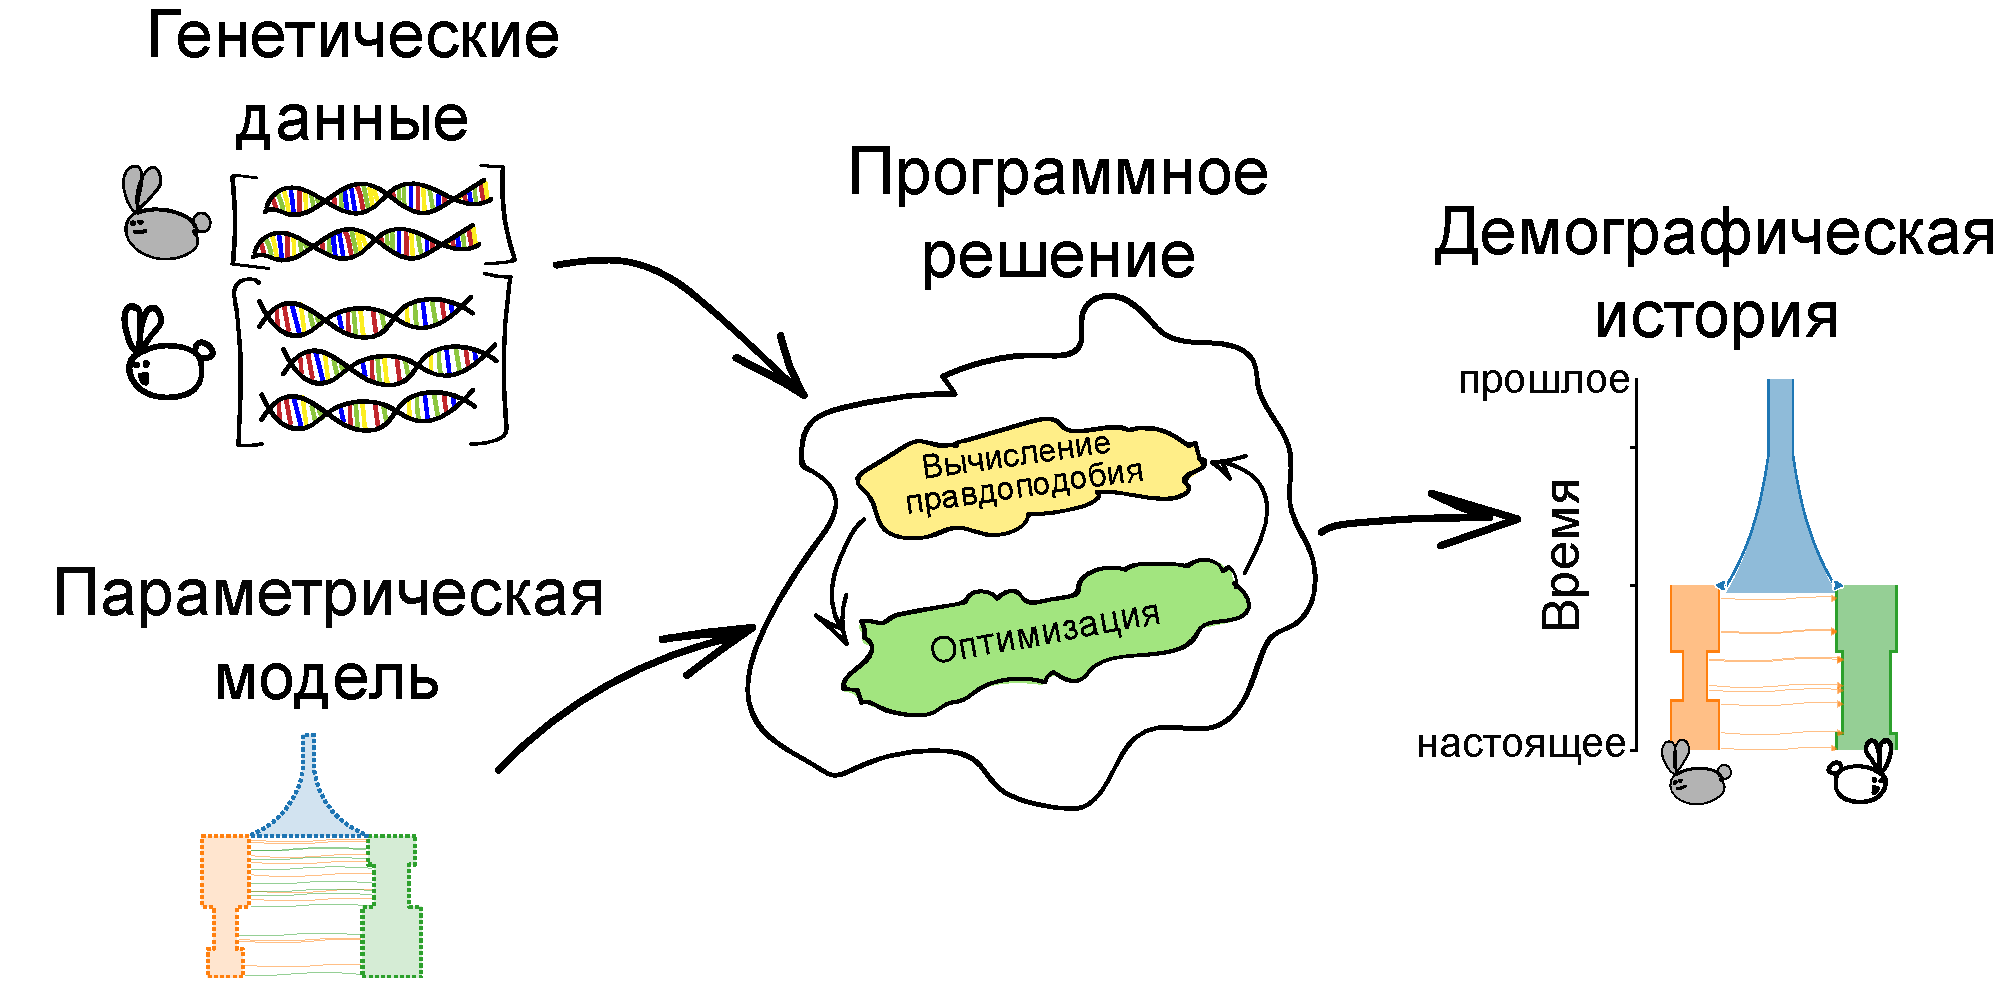
\includegraphics[width=0.6\textwidth]{images/part1/dem_history/general_scheme.pdf}
    \caption{Пример входа и выхода существующих программных решений для вывода демографической истории популяций по генетическим данным}
    \labelsyn{fig:part1:deminf:general_scheme}
\end{figure}


В \textbf{разделе 1.3} описаны два класса моделей демографических историй, которые применяются в существующих решениях, а также методы сравнения моделей с разным числом параметров.

\textit{Модели первого класса} используются в программных решениях \dadi, \moments и \momentsLD.
Они представляются в виде последовательности элементов временных интервалов, разделений, единичных миграций и элементов инбридинга (рисунок~\ref{fig:dadi:model_spec}).
Они имеют только непрерывные параметры, а динамики изменения численности (константная численность, линейное или экспоненциальное изменение) в этих моделях всегда фиксированы.

\begin{figure}[b]
    \centering
    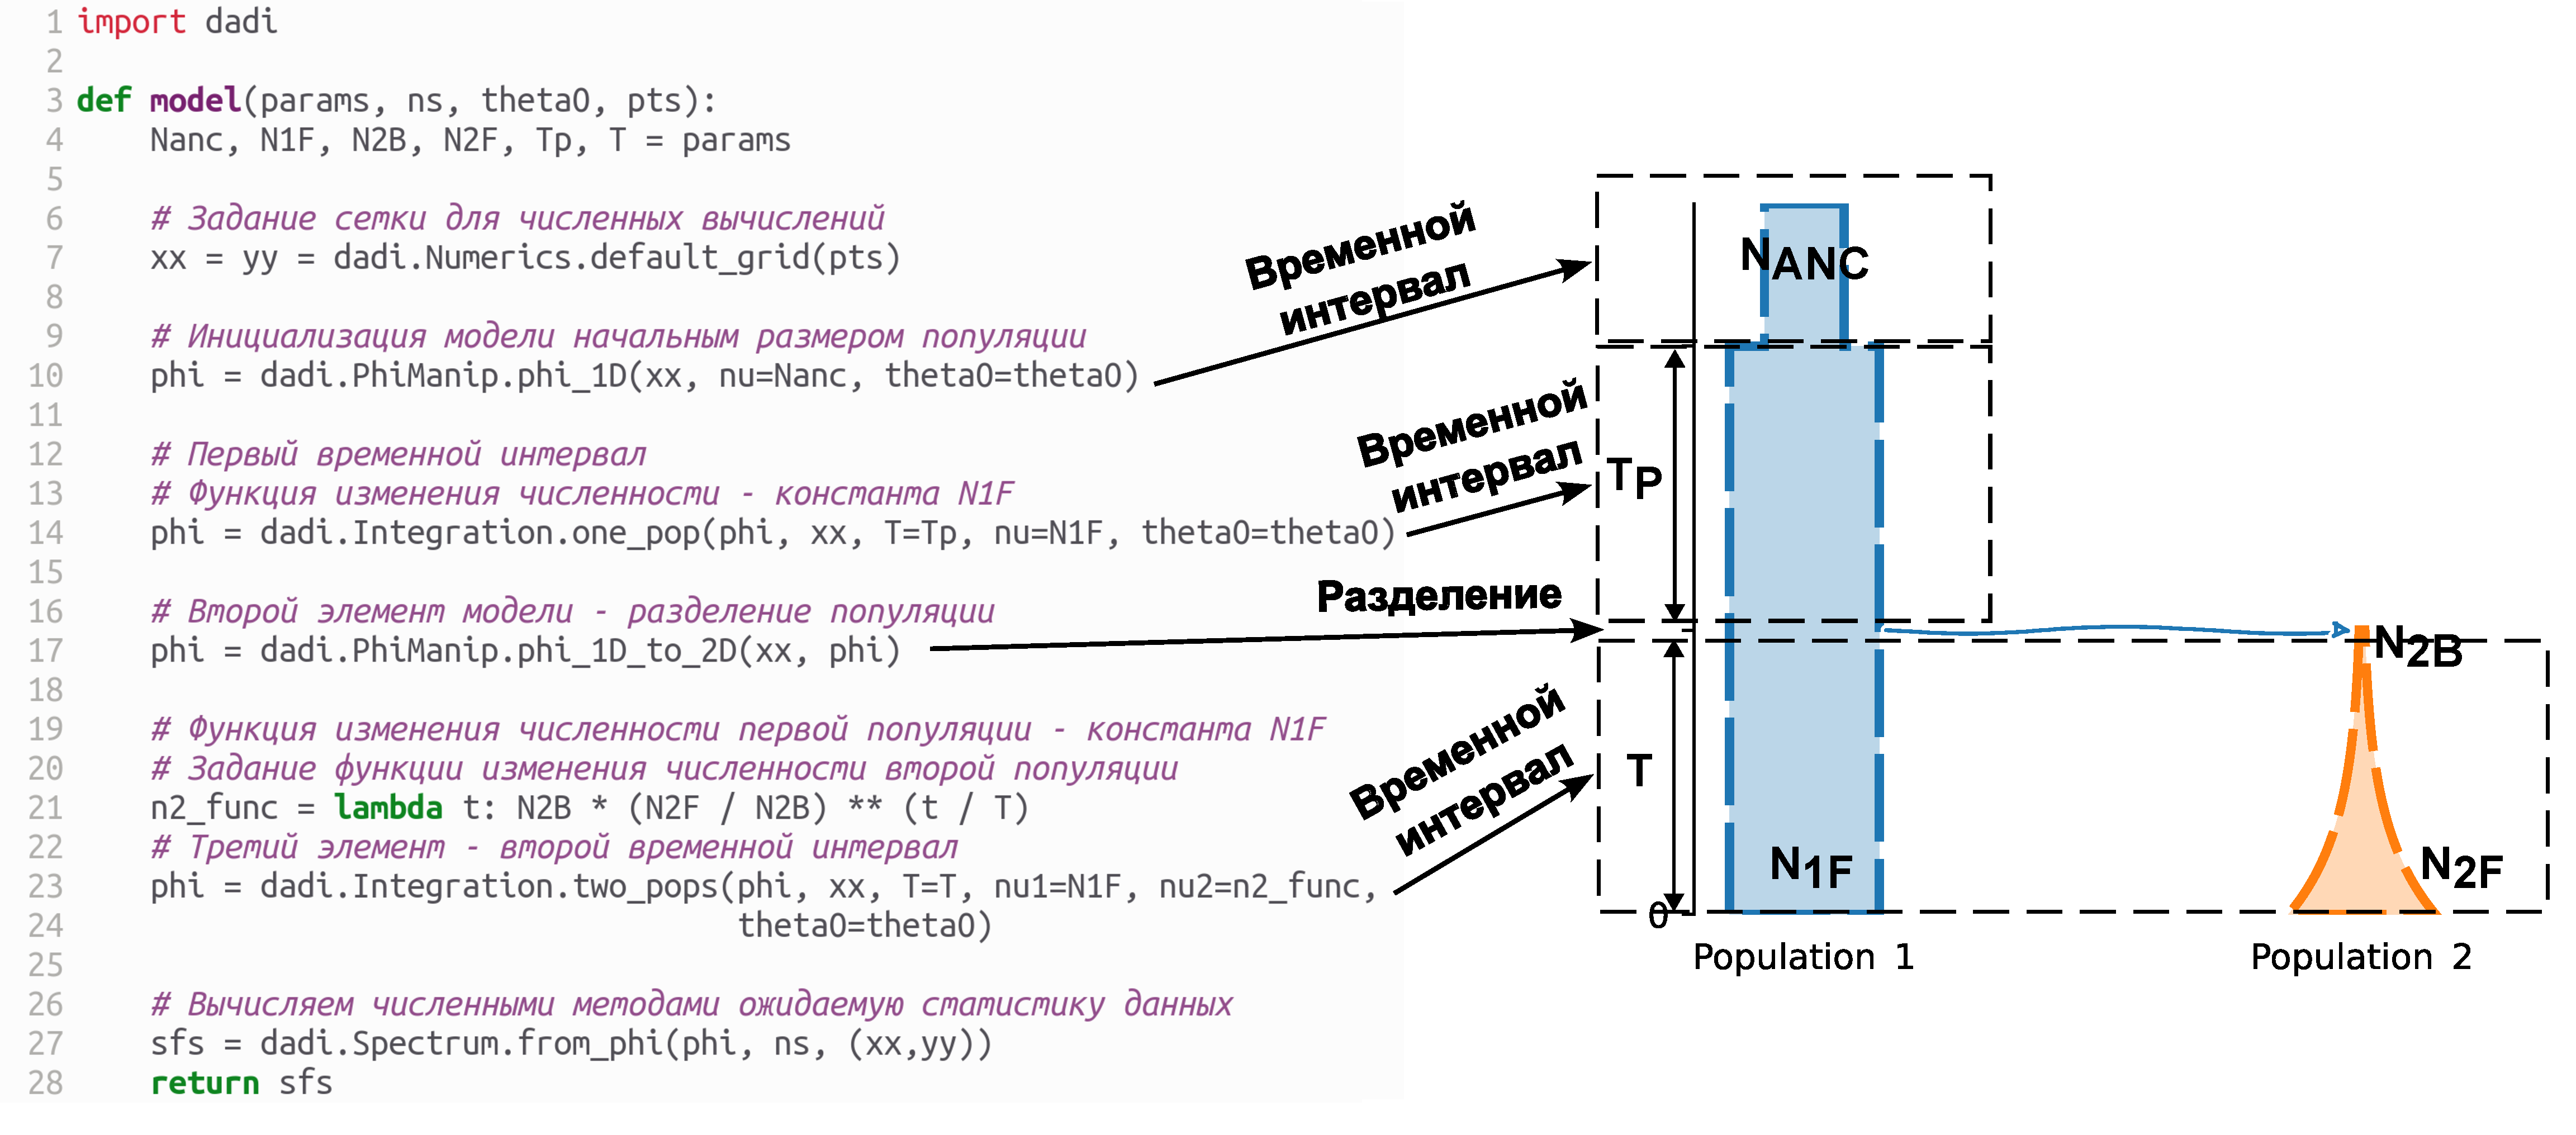
\includegraphics[width=\linewidth]{images_2/dadi_model.pdf}
    \caption{Пример задания модели первого класса с использованием интерфейса библиотеки~\dadi}
    \labelsyn{fig:dadi:model_spec}
\end{figure}


\textit{Модели второго класса} применяются в программном решении \momi.
Они представляются в виде набора событий изменения численности, разделения популяций и единичных миграций.
Модели второго класса также включают только непрерывные параметры и имеют фиксированные динамики изменения численности.
Однако они являются более ограниченными по сравнению с моделями первого класса, например, не поддерживают линейное изменение численности или непрерывные миграции.

Проблема выбора модели в общем случае состоит в том, что необходимо выбрать наиболее подходящую модель для данных.
Если выбрана слишком простая модель --- с малым числом параметров, она может не отображать всю информацию из данных.
Если выбрана слишком сложная модель --- с большим числом параметров, она может переобучиться на шуме в данных и в итоге неправильно моделировать реальный процесс.
Для сравнения различных моделей и выбора наилучшей используют  информационный критерий Акаике (AIC)~\cite{akaike1974new}, байесовский информационный критерий (BIC)~\cite{schwarz1978estimating} и тест отношения правдоподобия~\cite{vuong1989likelihood}.

В \textbf{разделе 1.4} приведено описание существующих методов вычисления правдоподобия генетических данных при условии заданной демографической истории.
В раздел включены определения основных понятий биологии и генетики, например, ДНК, генов, аллелей и генотипов.
Также описаны основные используемые статистики данных: аллель-частотный спектр и статистики на основе неравномерного сцепления генов.
Наконец, приведено описание методов вычисления правдоподобия, реализованных в программных решениях \dadi, \moments, \momi и \momentsLD.

\textbf{Раздел 1.5} содержит общее описание методов локальной и глобальной оптимизации, основные отличия этих двух групп, а также обзор существующих методов оптимизации для настройки параметров моделей демографических историй по генетическим данным.
Преимущественно применяются методы локальной оптимизации такие, как метод Бройдена-Флетчера-Гольдфарба-Шанно (BFGS)~\cite{broyden1970convergence,fletcher1970new, goldfarb1970family,shanno1970conditioning}, метод Нелдера-Мида~\cite{nelder1965simplex} и метод Пауэлла~\cite{powell1964efficient}~(рисунок~\ref{fig:syn_ru:opt:opt_example}).
% Программные решения \textit{dadi pipeline}~\cite{portik2017evaluating} и \textit{moments pipeline}~\cite{leache2019exploring} реализуют алгоритм последовательных раундов метода Нелдера-Мида для оптимизации функции правдоподобия \dadi и \moments соответственно.
% Также после первой нерецензируемой публикации диссертанта в 2019 году в \dadi был реализован первый алгоритм глобальной оптимизации BOBYQA~\cite{powell2009bobyqa, blischak2020inferring}.
Существующие методы оптимизации для настройки параметров моделей ограничены выводом значений только непрерывных параметров и требуют вовлечения пользователя для задания начальных значений параметров модели и гиперпараметров метода, например, числа перезапусков.
Использование методов локальной оптимизации не гарантирует нахождение глобального оптимума.

\begin{figure}[hb]
    \begin{subfigure}[b]{\linewidth}
    \centering
    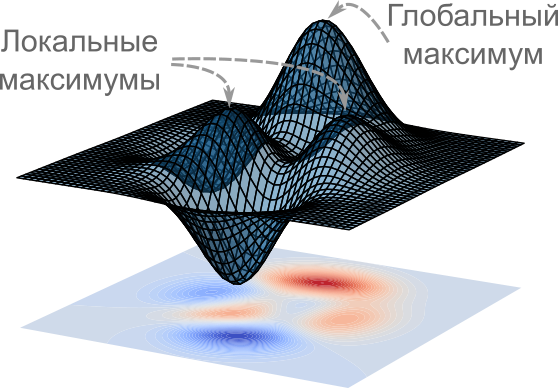
\includegraphics[height=3.2cm]{images/part1/opt/example_3d.png}
    \caption{}
    \labelsyn{fig:syn_ru:opt:opt_example_3d}
    \end{subfigure}
    \begin{subfigure}[b]{.33\linewidth}
    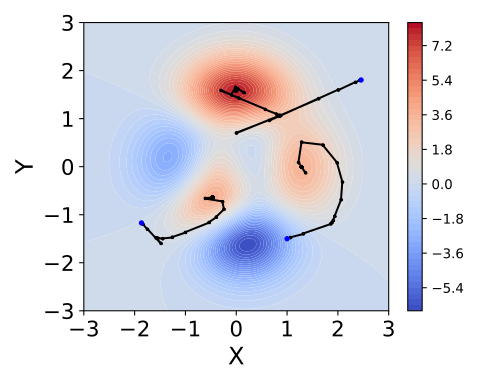
\includegraphics[height=3.2cm]{images/part1/opt/example_bfgs.png}
    \caption{}
    \labelsyn{fig:syn_ru:opt:opt_example_bfgs}
    \end{subfigure}%
    \begin{subfigure}[b]{.33\linewidth}
    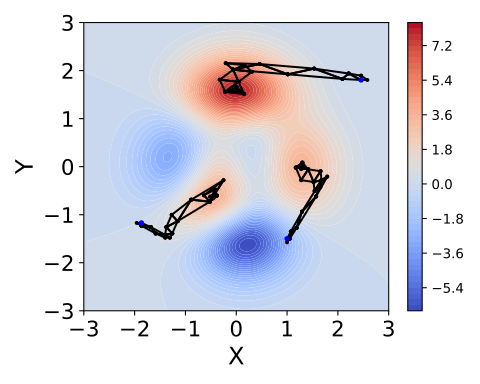
\includegraphics[height=3.2cm]{images/part1/opt/example_nelder_mead.png}
    \caption{}
    \labelsyn{fig:syn_ru:opt:opt_example_nelder_mead}
    \end{subfigure}%
    \begin{subfigure}[b]{.33\linewidth}
    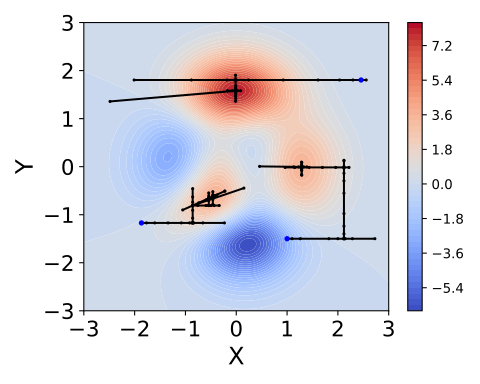
\includegraphics[height=3.2cm]{images/part1/opt/example_powell.png}
    \caption{}
    \labelsyn{fig:syn_ru:opt:opt_example_powell}
    \end{subfigure}
    \caption{Примеры работы методов локальной оптимизации при поиске максимума функции, изображенной на рисунке (а): (б) метод BFGS, (в) метод Нелдера-Мида, (г) метод Пауэлла.}
    \labelsyn{fig:syn_ru:opt:opt_example}
\end{figure}

В \textbf{разделе 1.6} приведены существующие методы перебора моделей демографической истории популяций, а также модификации подходов сравнения моделей с разным числом параметров в условиях зависимости генетических данных.
На момент начала исследований в 2017 году не существовало метода автоматического перебора моделей демографической истории популяций.
Все сравнения моделей проводились пользователем вручную с использованием информационного критерия Акаике или теста отношения правдоподобия.
После публикации первой статьи~\cite{noskova2020gadma} диссертанта появилось единственное программное средство~\cite{rippe2021environmental}, реализующее аналог метода автоматического перебора моделей.
Однако он ограничен анализом двух популяций и предполагает независимость данных.
В общем случае, генетические данные имеют зависимости: определенные части генома наследуются вместе.
Если данные зависимы, то информационный критерий Акаике и тест отношения правдоподобия будут ошибочно отдавать предпочтение моделям с большим числом параметров~\cite{gao2010composite}.
Существующие модификации этих конструкций~\cite{coffman2016computationally} позволяют учитывать эти зависимости.



Во \underline{\textbf{второй главе}} описаны разработанный расширенный класс моделей демографических историй, методы настройки их параметров на основе комбинации методов глобальной и локальной оптимизации, а также экспериментальные исследования разработанных моделей и методов.

\textbf{Раздел 2.1} содержит описание разработанного класса расширенных моделей демографической истории, реализацию этих моделей и примеры использования.
В качестве прототипа был выбран первый класс моделей.
Разработанные модели включают новый тип параметров для настройки --- дискретные параметры динамики изменения численности, которые могут представляться одной из трех зависимостей: постоянная численность, линейное или экспоненциальное изменение.
Изображение предложенной модели, а также демографические истории при разных значениях параметра \texttt{Dyn} показаны на рисунке~\ref{fig:new_model:model}.

\begin{figure}[ht]
    \centering
    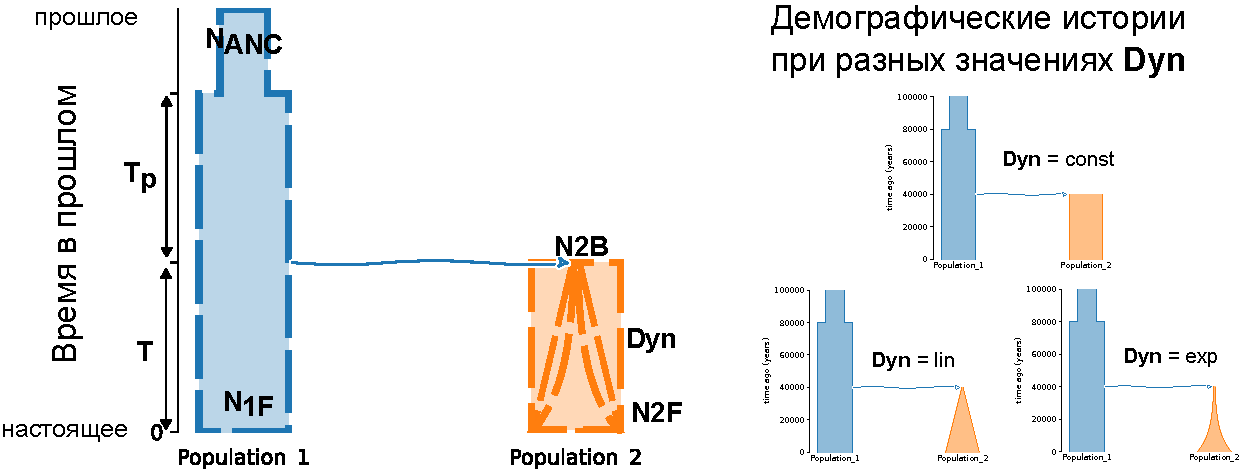
\includegraphics[width=\linewidth]{images_2/picture_2pops_model_3.pdf}
    \caption{Пример расширенной модели демографической истории двух популяций и демографические истории при разных значениях параметра \texttt{Dyn}}
    \labelsyn{fig:new_model:model}
\end{figure}



В \textbf{разделе 2.2} приведено формальное описание разработанного метода настройки параметров моделей расширенного класса на основе комбинации генетического алгоритма и метода локального поиска.
Описаны общая схема, разработанные операторы мутации и скрещивания в генетическом алгоритме, реализация и примеры применения предложенного метода.
Кроме того, в разделе приведены результаты автоматической настройки гиперпараметров генетического алгоритма для более эффективного решения поставленной задачи.

\textbf{Раздел 2.3} описывает второй разработанный метод настройки параметров моделей расширенного класса --- на основе комбинации байесовской оптимизации и метода локального поиска.
Приведено описание байесовской оптимизации и ее компонент, существующего метода кросс-валидации для выбора некоторых гиперпараметров, а также реализации разработанного метода.
Как и в случае с генетическим алгоритмом, были настроены гиперпараметры байесовской оптимизации.
Проведены экспериментальные исследования для ручной настройки, на основе которых была предложена ансамблевая байесовская оптимизация.

\textbf{Раздел 2.4} включает экспериментальные исследования разработанного метода настройки параметров на основе комбинации генетического алгоритма и локального поиска.

Сначала были проведены экспериментальные исследования разработанного метода в сочетании с методом вычисления правдоподобия, реализованным в \moments.
Проведено сравнение разработанного метода с методом Пауэлла с перезапусками и методом последовательных запусков метода Нелдера-Мида, реализованным в \textit{moments-pipeline}.
Для сравнения использовались модели первого класса и три набора симулированных данных.
Сравнение показало, что разработанный метод (GA) позволяет более эффективно настраивать параметры моделей (таблица~\ref{tab:part2:experiments:simulated_3:results}).
Дополнительно были рассмотрены предложенные расширенные модели и была проведена настройка их параметров с использованием разработанного метода.
Метод позволил корректно настроить параметры расширенных моделей, включая динамики изменения численности популяций.

\begin{table}[bh!]
    \caption{Результаты экспериментальных исследований сравнения методов настройки параметров на симулированных данных трех популяций}
    \resizebox{\linewidth}{!}{
    \begin{tabular}{|l | c | c | c |}
    \hline
    & Метод Пауэлла  & \multirow{2}{*}{\textit{moments-pipeline}} & \multirow{2}{*}{GA}\\
    & с перезапусками & & \\ 
    \hline
    Среднее число вычислений &  $22{\,}475$ & $19{\,}452$ & $21{\,}651$ \\
    \hline
    Среднее $f^{\text{\moments}}$ &$-11{\,}178{,}62$ & $-11{\,}179{,}82$ & $\mathbf{-11{\,}178{,}45}$\\
    \hline
    Стандартное & $0{,}40$ & $0{,}72$ & $\mathbf{0{,}15}$\\
    отклонение $f^{\text{\moments}}$ & & & \\
    \hline 
    Лучшее $f^{\text{\moments}}$ & $-11{\,}178{,}31$ & $-11{\,}178{,}59$ & $\mathbf{-11{\,}178{,}29}$\\
    \hline
    \end{tabular}%
    }
    \labelsyn{tab:part2:experiments:simulated_3:results}
\end{table}


Затем были проведены три экспериментальных исследования разработанного метода в сочетании с методом вычисления правдоподобия, реализованным в \dadi.

Метод был применен для реальных данных популяций кошачьей лягушки (\textit{Scotobleps gabonicus}), которые ранее были проанализированы в~\cite{portik2017evaluating} с применением \textit{dadi-pipleine}.
Для трех различных пар популяций были получены демографические истории с использованием тех же 12 моделей, которые были использованы в~\cite{portik2017evaluating}.
Для 92\% моделей разработанный метод нашел параметры с большим значением правдоподобия, чем было получено с применением \textit{dadi-pipleine}.
В 5\% случаев правдоподобие совпало и только для одной модели (3\%) оно оказалось хуже.

На данных двух популяций американской пумы (\textit{Puma concolor}) разработанный метод был сравнен с методом BFGS с перезапусками и методов BOBYQA с перезапусками.
Использовались две модели, предложенные и проанализированные ранее в работе~\cite{blischak2020inferring}, без инбридинга и с инбридингом.
Показано, что разработанный метод в среднем оказывается более эффективным, чем методы BFGS и BOBYQA (таблица~\ref{tab:part2:experiments:puma:puma_F_res}).
Дополнительная настройка параметров моделей с использованием расширенной области значений параметров позволила получить демографическую историю, имеющую значение правдоподобия выше, чем было получено ранее.

\begin{table}[ht]
    \centering
    \caption{Результаты 100 запусков различных методов для поиска параметров модели с инбридингом для вывода демографической истории двух популяций пум}
    \resizebox{\linewidth}{!}{%
    \begin{tabular}{|p{3.3cm}|P{1.9cm}|P{1.9cm}|P{1.9cm}|P{1.9cm}|P{1.9cm}|}
         \hline
         & \multicolumn{2}{c|}{BFGS} &  \multicolumn{2}{c|}{BOBYQA} & GA \\
         &  1 запуск & 16 запусков & 1 запуск & 4 запуска &\\
         \hline
         Число вычислений правдоподобия & $394\pm82$ & $6{\,}245\pm324$ & $1{\,}605 \pm 1{\,}207$ & $6{\,}095 \pm 2{\,}561$ & $6{\,}193\pm2{\,}680$ \\
         \hline
         Время CPU (мин.) &  $1{,}3\pm1{,}4$ & $25\pm19$ & $ 12\pm 5$ & $16\pm7$ & $93\pm47$ \\
         \hline
         Лучшее правдоподобие &  $-317{\,}370{,}88$ & $-317{\,}370{,}88$ & $\mathbf{-317{\,}239{,}48}$ & $\mathbf{-317{\,}239{,}48}$ & $-317{\,}239{,}49$ \\
         \hline
         Среднее правдоподобие &  $-1{\,}729{\,}870$ & $-320{\,}947$ & $-381{\,}979$ & $-320{\,}503$ & $\mathbf{-319{\,}451}$ \\
         \hline
         Стандартное отклонение правдоподобия & $4{\,}339{\,}276$ & $5{\,}029$ & $115{\,}205$ & $8{\,}753$ & $7{\,}340$ \\
         \hline
    \end{tabular}%
    }
    \labelsyn{tab:part2:experiments:puma:puma_F_res}
\end{table}

Аналогичным образом разработанный метод был сравнен с методом BOBYQA с перезапусками на данных огородной капусты (\textit{Brassica oleracea}), которые ранее были   проанализированы в работе~\cite{blischak2020inferring}.
На этих данных метод BOBYQA с множественными запусками показал результаты лучше, чем разработанный метод, однако, отметим, что число перезапусков, необходимых для достижения эффективности метода BOBYQA, остается неизвестным в общем случае.
Было рассмотрено расширенное пространство значений параметров, что позволило получить демографические истории, имеющие лучшее значение правдоподобия, чем получено ранее.

Затем, четыре существующих метода вычисления правдоподобия, реализованные в \dadi, \moments, \momi и \momentsLD, были сравнены с использованием разработанного метода на данных орангутанга, симулированных с использованием библиотеки \textit{stdpopsim}~\cite{adrion2020community,lauterbur2023expanding}.
Сравнение было проведено с применением различных моделей, включая модели расширенного класса.
Было показано, что все методы позволяют восстановить исходную демографическую историю при применении корректных моделей.
Использование моделей, которые не способны отразить исходную историю, например, не включающих непрерывные миграции, приводит к различиям в получаемых результатах (рисунок~\ref{fig:part2:experiments:sim2:results:oran_momi}).
Однако отметим, что основные характеристики популяций такие, например, как численность, настраиваются корректно и в таком случае.

\begin{figure}[ht]
    \centering
    \begin{subfigure}[b]{0.24\linewidth}
        \centering
        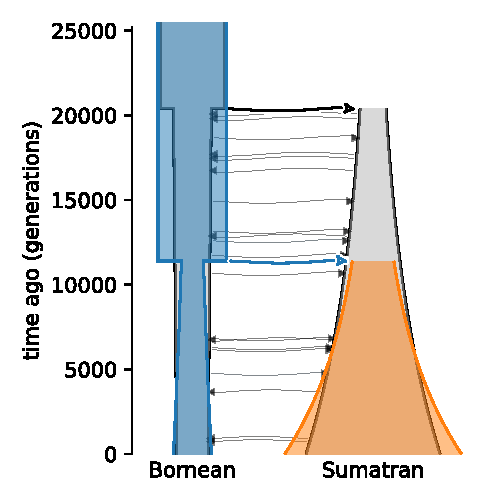
\includegraphics[width=\textwidth]{images_experiments/suimulation_2_stdpopsim/ORAN-PULSE/oran-nomig.pdf}
        \caption{}
        \labelsyn{fig:part2:experiments:sim2:results:oran_momi_nomig}
    \end{subfigure}%
    \begin{subfigure}[b]{0.24\linewidth}
        \centering
        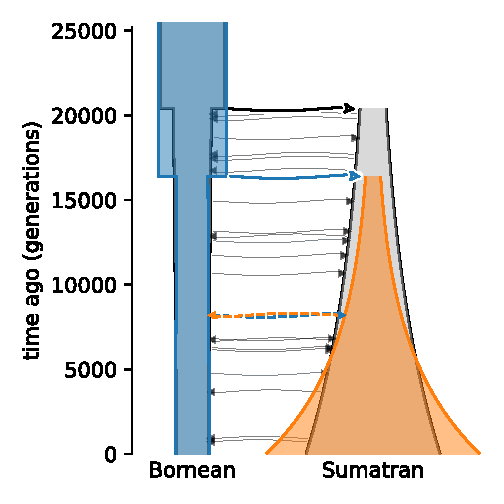
\includegraphics[width=\textwidth]{images_experiments/suimulation_2_stdpopsim/ORAN-PULSE/oran-pulse-1.pdf}
        \caption{}
        \labelsyn{fig:part2:experiments:sim2:results:oran_pulse_1}
    \end{subfigure}%
    \begin{subfigure}[b]{0.24\linewidth}
        \centering
        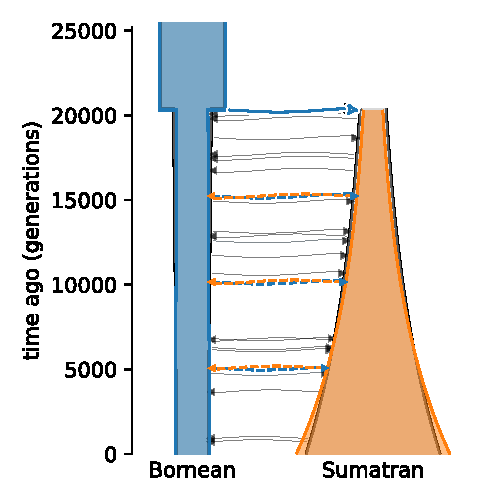
\includegraphics[width=\textwidth]{images_experiments/suimulation_2_stdpopsim/ORAN-PULSE/oran-pulse-3.pdf}
        \caption{}
        \labelsyn{fig:part2:experiments:sim2:results:oran_pulse_3}
    \end{subfigure}%
    \begin{subfigure}[b]{0.24\linewidth}
        \centering
        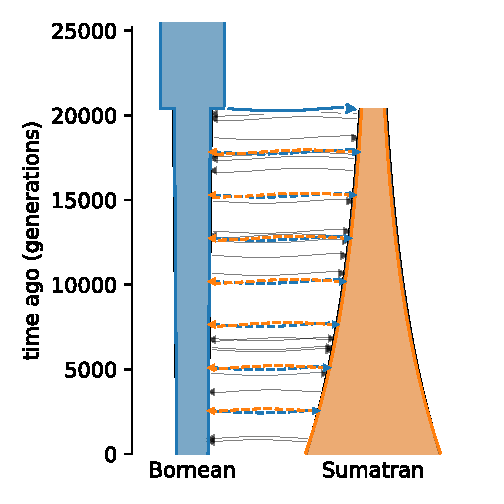
\includegraphics[width=\textwidth]{images_experiments/suimulation_2_stdpopsim/ORAN-PULSE/oran-pulse-7.pdf}
        \caption{}
        \labelsyn{fig:part2:experiments:sim2:results:oran_pulse_7}
    \end{subfigure}
    \caption{Результаты настроенных моделей для метода вычисления правдоподобия, реализованного в \momi (а)~модель без миграций, и модели с (б)~одной, (в)~тремя, (г)~семью единичными миграциями}
    \labelsyn{fig:part2:experiments:sim2:results:oran_momi}
\end{figure}

Наконец, была выведена демографическая история трех популяций современного человека на территории России: жителей Пскова, Новгорода и Якутии.
Используемые данные ранее не были проанализированы.
Параметры расширенной модели были настроены с помощью разработанного метода на основе комбинации генетического алгоритма и локального поиска.
Полученная демографическая история (рисунок~\ref{fig:part2:experiments:rus:result}) согласуется с известной историей современного человека~\cite{schraiber2015methods, nielsen2017tracing}.

\begin{figure}[hb]
    \centering
        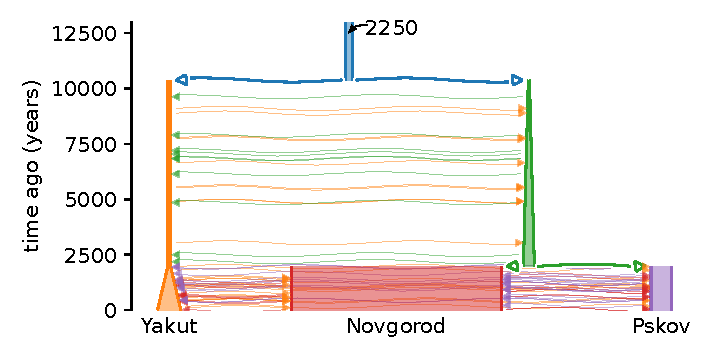
\includegraphics[width=0.7\linewidth]{images_experiments/rus_genomes/picture_result.pdf}
    \caption{Полученная демографическая история трех популяций современного человека}
    \labelsyn{fig:part2:experiments:rus:result}
\end{figure}

\textbf{Раздел 2.5} описывает результаты экспериментальных исследований разработанного метода настройки параметров моделей на основе комбинации байесовской оптимизации и локального поиска.

Байесовская оптимизация была сравнена с генетическим алгоритмом  на множестве наборов данных (рисунок~\ref{fig:bo_ga_comp}).
Было показано, что генетический алгоритм (GA) оказывается более эффективным в случае одной, двух и трех популяций.
Байесовская оптимизация (BO) имеет более быструю сходимость, чем генетический алгоритм, если рассматривается более трех популяций.
Применение байесовской оптимизации позволяет сократить время настройки параметров моделей на 50-80\%, что приводит к значительному ускорению процесса на дни и даже недели.

\begin{figure}[ht]
    \centering
    \begin{subfigure}[b]{0.49\linewidth}
        \centering
        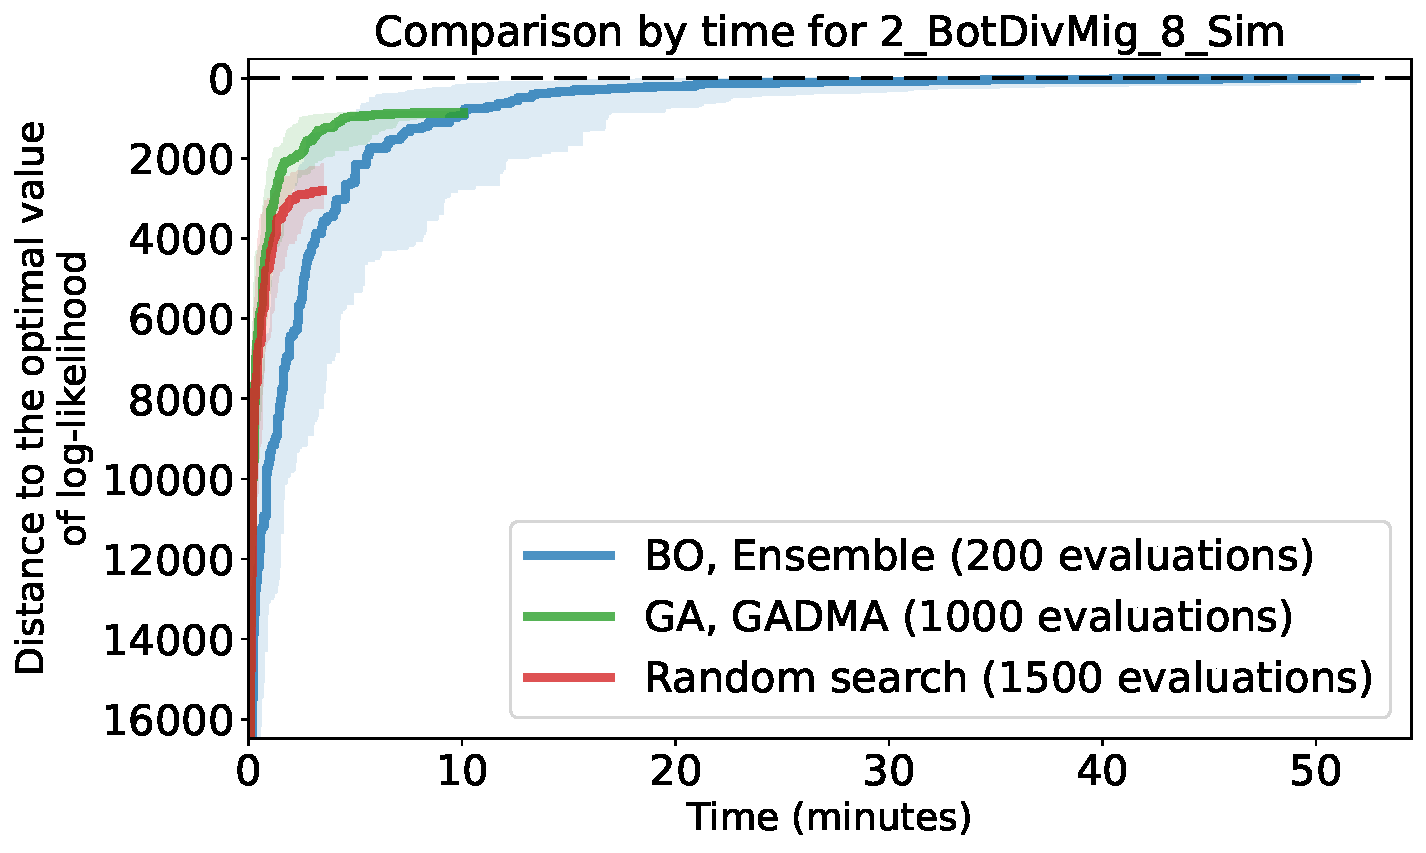
\includegraphics[width=0.87\textwidth]{images_experiments/bo_ga/2_BotDivMig_8_Sim_bo_ga_time.pdf}
        \caption{}
        \labelsyn{fig:bo_ga_comp:2pops}
    \end{subfigure}%
    \begin{subfigure}[b]{0.49\linewidth}
        \centering
        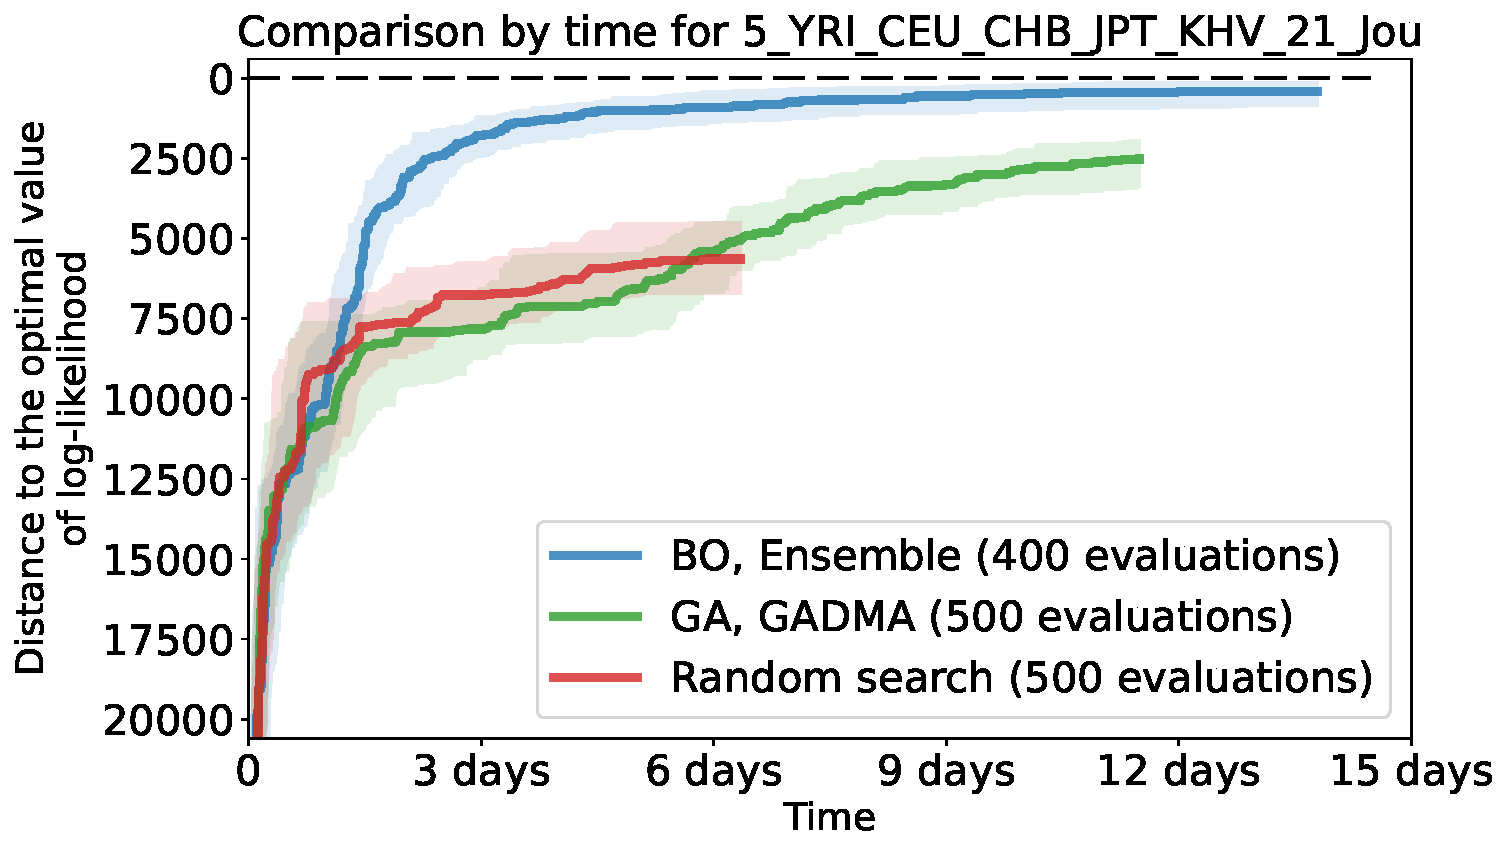
\includegraphics[width=0.87\textwidth]{images_experiments/bo_ga/5_YRI_CEU_CHB_JPT_KHV_21_Jou_bo_ga_time.pdf}
        \caption{}
        \labelsyn{fig:bo_ga_comp:5pops}
    \end{subfigure}
    \caption{Сходимость по времени методов настройки параметров моделей для (а) двух популяций, (б)~пяти популяций}
    \labelsyn{fig:bo_ga_comp}
\end{figure}

Также разработанный метод на основе комбинации байесовской оптимизации и метода локального поиска был использован для настройки параметров моделей демографических историй четырех и пяти популяций современного человека по реальным данным из статьи~\cite{jouganous2017inferring}.
Разработанный метод позволил получить параметры, которые дают лучшее значение правдоподобия, чем найденные в~\cite{jouganous2017inferring} с помощью метода Пауэлла с перезапусками.
Сравнение полученной демографической истории с более высоким значением правдоподобия и истории, полученной в оригинальной статье, представлено на рисунке~\ref{fig:syn_ru:bo_human}.
\begin{figure}[h!]
    \centering
    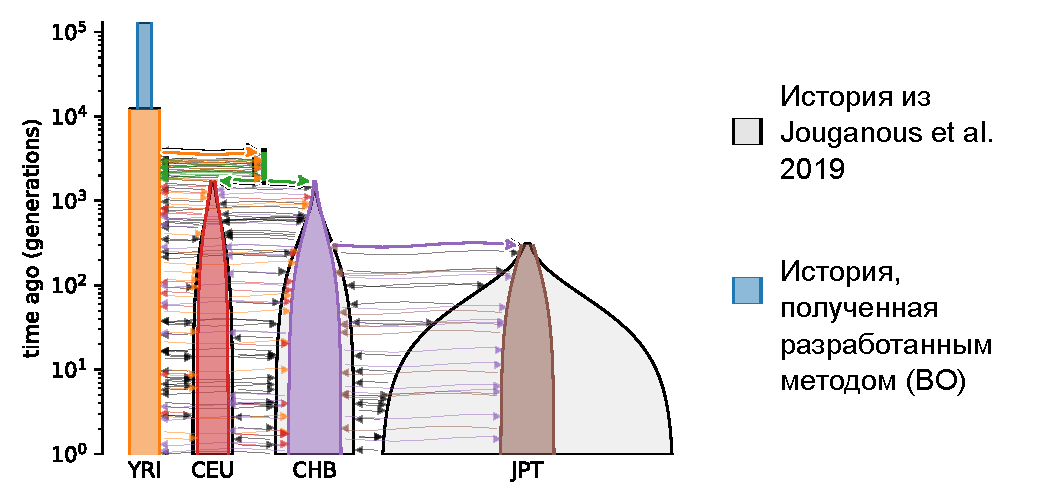
\includegraphics[width=0.8\linewidth]{images_experiments/bo_human/4pops_base.pdf}
    \caption{Сравнение демографической истории, полученной разработанным методом (BO), и демографической истории из~\cite{jouganous2017inferring}}
    \labelsyn{fig:syn_ru:bo_human}
\end{figure}


В \underline{\textbf{третьей главе}} описан разработанный метод автоматического перебора расширенных моделей демографической истории одной, двух и трех популяций, а также результаты его применения в сочетании с разработанным методом на основе комбинации генетического алгоритма и локального поиска.

В \textbf{разделе 3.1} приведено формальное описание разработанного метода.
На вход подаются минимальные и максимальные ограничения на модель.
На первом раунде метод строит модель, удовлетворяющую минимальным ограничением и выполняет настройку ее параметров с применением разработанного метода на основе генетического алгоритма.
На каждом следующем раунде происходит изменение модели, увеличение числа ее параметров и последующая настройка нового набора параметров.
Работа метода останавливается, когда модель достигает максимальных ограничений.
В конце происходит сравнение всех перебранных моделей с использованием информационного критерия Акаике и выбирается наилучшая.
В качестве ограничений на модели было предложено число временных интервалов.

В \textbf{разделе 3.2} приведены экспериментальные исследования разработанного метода автоматического перебора моделей.
Для генетических данных трех популяций современного человека была получена демографическая история «выхода из Африки», представленная на рисунке~\ref{fig:part4:experiments:3pop_human:result}.
Она согласуется с другими исследованиями~\cite{gutenkunst2009inferring, schraiber2015methods, nielsen2007recent} и имеет не только наилучшее значение правдоподобия, чем история, полученная ранее в~\cite{gutenkunst2009inferring} по тем же данным, но и лучшее значение информационного критерия Акаике.

\begin{figure}[ht]
    \centering
        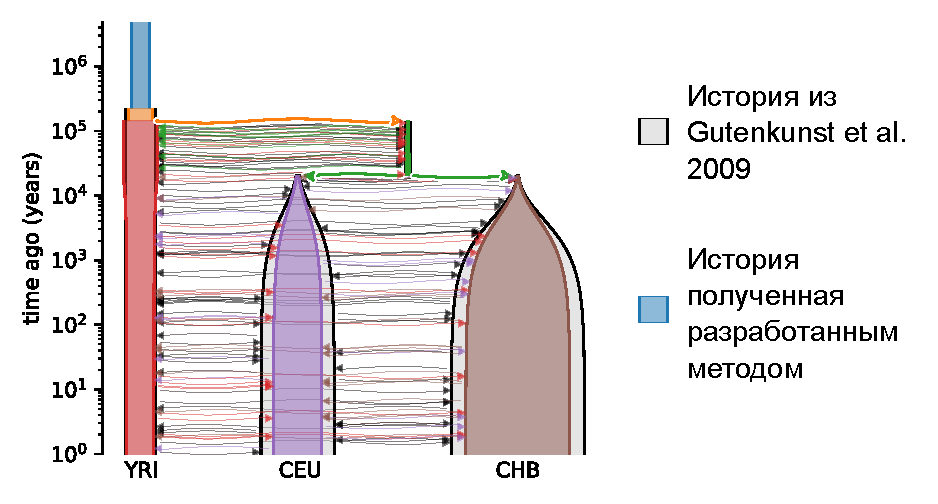
\includegraphics[width=0.8\textwidth]{images_experiments/3pop_human_gutenkunst/picture_3pop_result.pdf}
    \caption{Демографическая история, полученная разработанным методом}
    \labelsyn{fig:part4:experiments:3pop_human:result}
\end{figure}

Для трех наборов генетических данных популяции кошачьей лягушки (\textit{Scotobleps gabonicus}), на которых были построены модели в разделе 2.4 данной работы с использованием метода ручного перебора, также были получены модели демографических историй с использованием разработанного метода автоматического перебора.
Из двух наборов данных полученные модели показали наилучшее значение информационного критерия Акаике среди всех рассмотренных конфигураций.
В случае третьего набора данных полученная модель имеет значение информационного критерия Акаике, которое хуже, чем у лучшей модели, полученной в результате ручного перебора. Тем не менее, результаты позволяют выявить излишний параметр модели, и исключение этого параметра из конфигурации приводит к наилучшему значению информационного критерия Акаике.

Разработанный метод автоматического перебора расширенных моделей был использован при выводе демографической истории популяций голубой акулы.
Генетические данные ранее не были проанализированы.
Был разработан подход последовательного вывода демографической истории двух и трех популяций, в результате которого была получена демографическая история, представленная на рисунке~\ref{fig:part2:experiments:blue_shark:3pop_hist}.
Полученные численности популяций согласуются с другими исследованиями~\cite{king2015genetic,verissimo2017world}.
Апробация результатов, проведенная коллегами из области зоологии, позволила предположить, что разделение северной и южной популяций произошло в связи с палеоклиматическими событиями в эпоху голоцена~\cite{leduc2010holocene,masson2013information,olsen2012variability}.

\begin{figure}[ht]
    \centering
        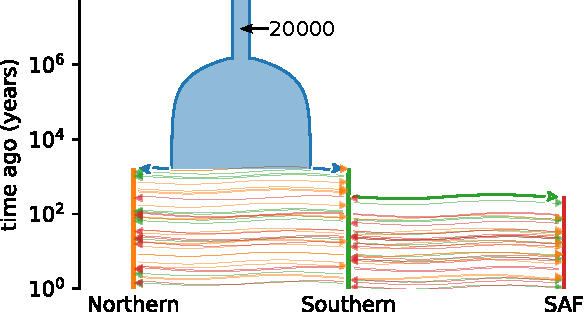
\includegraphics[width=0.6\linewidth]{images_experiments/blue_shark/3pop_history.pdf}
    \caption{Демографическая история трех популяций голубой акулы}
    \labelsyn{fig:part2:experiments:blue_shark:3pop_hist}
\end{figure}

В \underline{\textbf{четвертой главе}} приведено описание программных комплексов, которые реализовывают разработанные методы или были использованы в данной работе. 

\textbf{Раздел 4.1} содержит описание программного комплекса GADMA (Global seach Algorithm for Demographic Model Analysis), который реализует разработанные модели расширенного класса, методы настройки параметров этих моделей и метод автоматического перебора расширенных моделей.
Структура программного комплекса представлена на рисунке~\ref{fig:syn_ru:gadma_modules}.

\begin{figure}[ht]
    \centering
    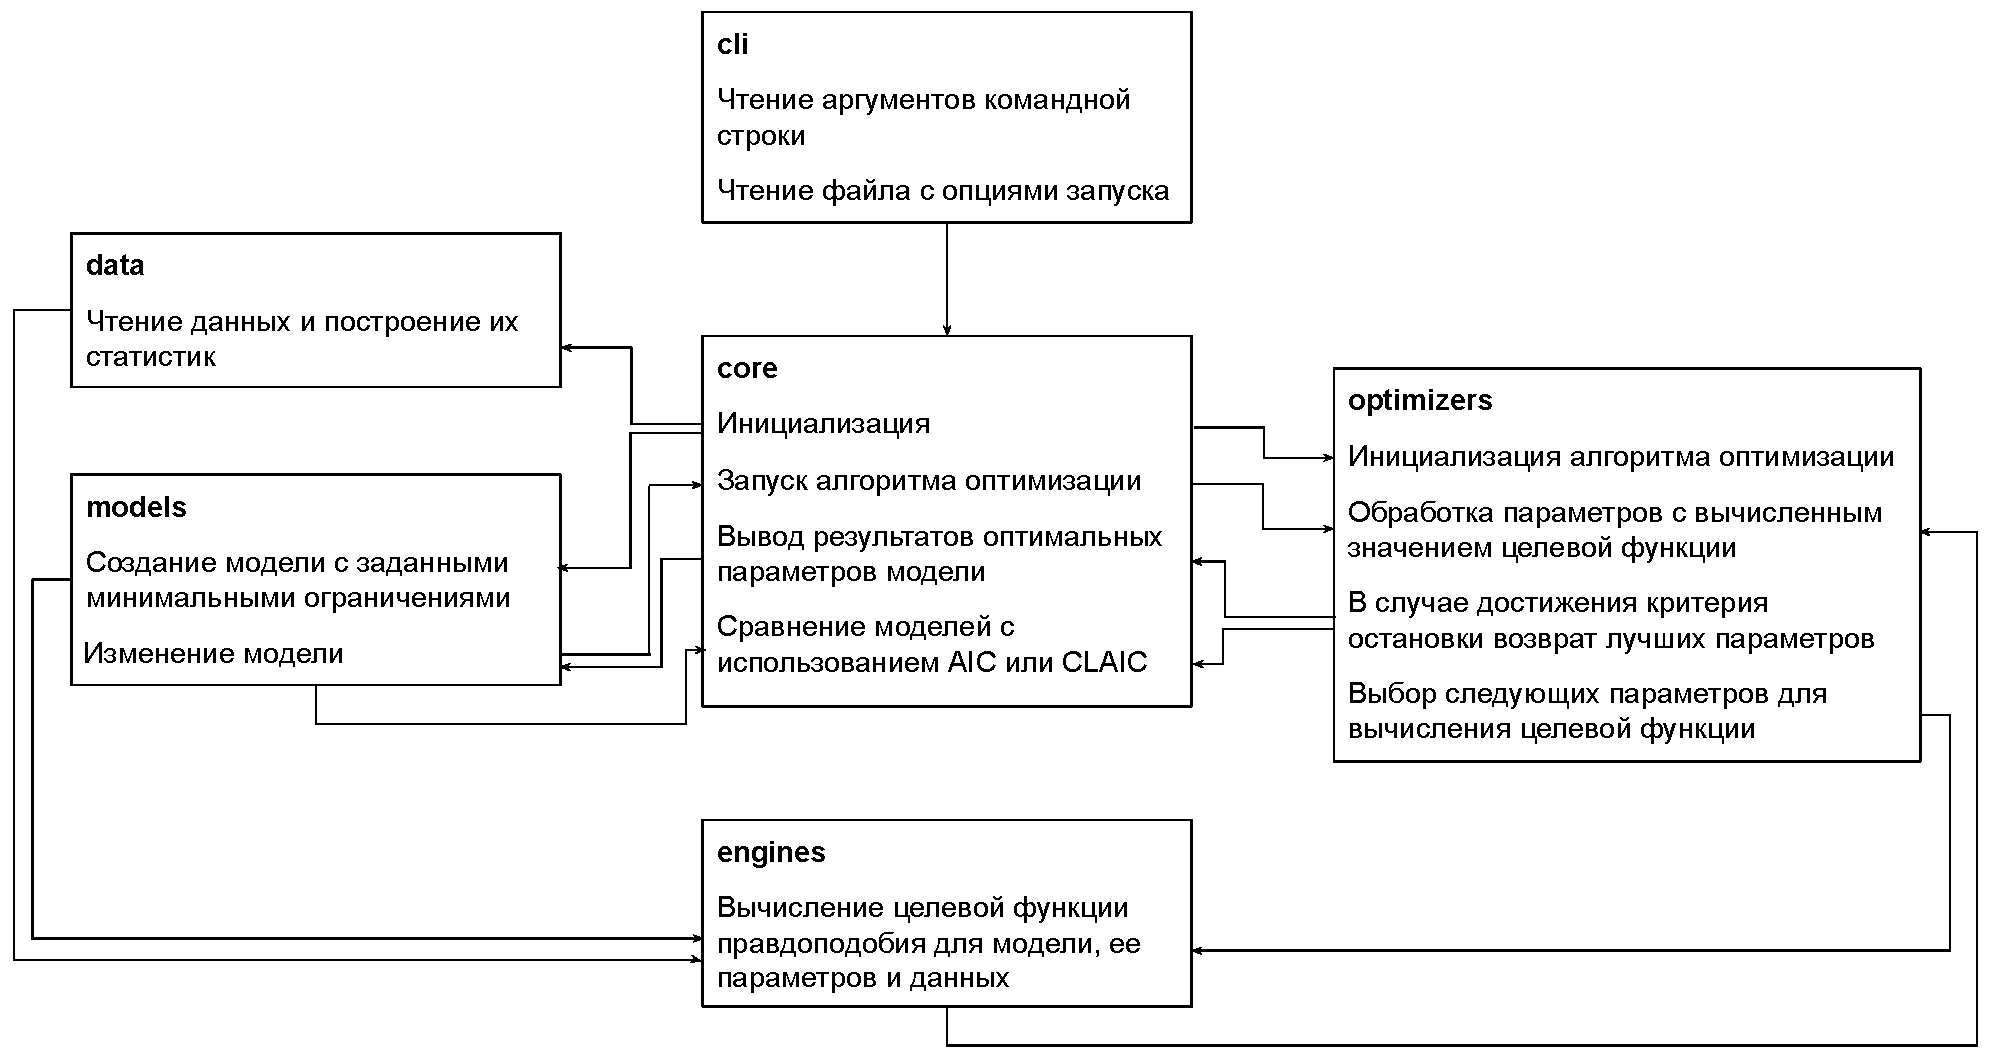
\includegraphics[width=\linewidth]{images/part5/gadma_modules.pdf}
    \caption{Структура программного комплекса GADMA}
    \labelsyn{fig:syn_ru:gadma_modules}
\end{figure}

В \textbf{разделе 4.2} приведено описание расширения библиотек \textit{stdpopsim} и \textit{demes}.
Библиотека \textit{stdpopsim} содержит каталог предопределенных видов и их демографических историй для более надежных симуляций генетических данных.
Эта библиотека была расширена и использована при проведении экспериментальных исследований.
Программное средство \textit{demes} предназначено для текстового и визуального представления демографических историй.
Эта библиотека была расширена реализацией линейного изменения численности популяции, а также была интегрирована в программный комплекс GADMA.
Все изображения демографических историй в данной диссертации были получены с использованием библиотеки \textit{demes}.

В \textbf{заключении} приведены основные результаты работы, которые состоят в следующем:
%!TEX root = ../dissertation.tex
\begin{itemize}
    \item проведено исследование текущего состояния предметной области, уточнение задачи и способов оценки результатов;
    \item формализована постановка задачи построения и настройки моделей метрических деревьев с функциями на ребрах на примере задачи вывода демографической истории популяций по генетическим данным;
    \item разработан метод автоматической настройки параметров моделей метрических деревьев с функциями на ребрах на основе комбинации методов глобальной и локальной оптимизации на примере задачи вывода демографической истории популяций по генетическим данным;
    \item разработан метод автоматического перебора моделей метрических деревьев с функциями на ребрах на примере задачи вывода демографической истории популяций по генетическим данным;
    \item спроектирован и реализован программный комплекс, включающий разработанные модели и методы для вывода демографической истории популяций по генетическим данным;
    \item проведены экспериментальные исследования, подтверждающие эффективность разработанных моделей и методов, а также их применимость для вывода демографической истории популяций по генетическим данным, проведен анализ результатов экспериментов.\\
\end{itemize}

Для оценки качества настройки моделей демографических историй в данной работе было использовано значение функции правдоподобия.
Результаты экспериментов показывают, что метод настройки параметров моделей на основе комбинации генетического алгоритма и локального поиска позволил в 88\% случаев (37 моделей из 42 протестированных) найти параметры модели, обеспечивающие лучшее значение правдоподобия, чем параметры, найденные существующими ранее методами.
На симулированных данных разработанный метод позволил найти решения, которые на 97\% ближе к оптимуму в случае одной популяции и на 66\% ближе к оптимуму в случае трех популяций, чем решения, полученные существующими методами.
Настройка гиперпараметров генетического алгоритма позволила ускорить реализацию в среднем на 10\% с сохранением эффективности метода.

Была подтверждена эффективность метода настройки параметров моделей на основе байесовской оптимизации и локальной оптимизации в условиях сложновычислимной целевой функции.
Разработанный метод позволил найти значения параметров, обеспечивающих лучшее значение правдоподобия, чем существующие методы, для двух ранее проанализированных данных четырех и пяти популяций.
Было показано, что байесовская оптимизация достигает решения, близкого к оптимуму, на 50-80\% быстрее, чем генетический алгоритм, в случае вывода демографической истории четырех и пяти популяций.

Метод автоматического перебора моделей позволяет автоматически строить и настраивать модели в заданных ограничениях на конфигурацию.
Сравнение моделей демографических историй с разным числом параметров было осуществлено с использованием информационного критерия Акаике (AIC).
Экспериментальные исследования показали, что в трех из четырех случаях метод позволил найти модель, обеспечивающую лучшее значение AIC, чем было получено ранее ручным перебором.
В четвертом случае, полученная модель позволила установить излишние параметры в конфигурации и построить вложенную модель, которая в итоге обеспечила наилучшее значение AIC для данных.

В качестве перспективных направлений исследования можно выделить совершенствование метода автоматического перебора моделей с целью поиска оптимального набора параметров конфигурации, а также разработку методов настройки моделей метрического дерева с функциями на ребрах, которые позволяют осуществлять настройку не только функциональных параметров, но и поиск оптимальной структуры дерева.